
\section{Project 8 - Morphological Processing}

\subsection{Project Proposal}
Implement the \emph{"Opening by reconstruction", "Filling holes" and "Border clearing"} operations on textbook \emph{chapter 9.5}. The task is to reproduce the results in \emph{Figure 9.29, 9.31 and 9.32}.

\subsection{Preliminaries}
\subsubsection{Basic morphological operations}
Morphology offers a unified and powerful approach to numerous image processing problem. These operations defined based on set theory. In this project we consider that morphological operations are conducted on binary images (preprocessing is required for gray-level images). The below table describes the basic widely used morphological processing.
\begin{table}[h]
	\caption{Summary of basic morphological operations.}
	\centering
	\begin{tabular}{|l|l|m{0.45\columnwidth}|}\hline
		Operation & Equation & Comments\\ \hline
		Translation & $(B)_z=\{w|w=b+z, ~ b \in B \}$ & Translation the origin of $B$ to point $z$.\\
		Reflection & $\hat{B}=\{w|w=-b, ~ b \in B\}$ & Reflects all elements of B about the origin of this set.\\
		Complement & $A^c=\{ w|w \notin A \}$ & Set of points not in $A$.\\
		Difference & $A-B=\{ w|w \in A, w \notin B\}$ & Set of points that belong to $A$ but not to $B$.\\
		Dilation & $A \oplus B=\left\{ z|(\hat{B}_z) \cap A \neq \emptyset \right\}$ & Expands the boundary of $A$.\\
		Erosion & $A \ominus B=\left\{ z|(B)_z \subseteq A \right\}$ & Contracts the boundary of $A$.\\
		Opening & $A \circ B=(A\ominus B)\oplus B $ & Smoothes contours, breaks narrow isthmuses, and eliminates small islands and sharp peaks.\\
		Closing & $A \bullet B=(A\oplus B)\ominus B $ & Smoothes contours, fuses narrow breaks and long thin gulfs and eliminates small holes.\\
		Hit-or-miss transform & $A \otimes B=(A\ominus B_1)\cap(A^c\ominus B_2)$ & The set of pints at which, simultaneously $B_1$ found a hit in $A$ and $B_2$ found a match in $A^c$.\\ \hline
	\end{tabular}
\end{table}

\subsubsection{Morphological restoration}
With the basic operations, we can discuss a powerful morphological transformation \emph{morphological restoration} that involves two images and a structuring element. One image, the \emph{marker}, contains the starting points for the transformation. The other image, the \emph{mask}, constrains the transformation. \\
\subsubsection*{Geodesic dilation and erosion}
Geodesic dilation and erosion are the central concepts to morphologic reconstruction. Let $F$ denote the maker and $G$ denote the mask and $F \subseteq G$. The \emph{geodesic dilation} of size 1 of the marker with respect to the mask, denoted by $D_G^(1)(F)$, is defined as 
\begin{equation} D_G^{(1)}(F)=(F\oplus B) \cap G \end{equation}
The geodesic dilation of size $n$ of $F$ with resplect to $G$ is defined as 
\begin{equation} D_G^{(n)}(F)=D_G^{(1)} \left[ D_G^{(n-1)}(F) \right]\end{equation}
with $D_G^{(0)}(F)=F$. Similarly, the \emph{geodesic erosion} of size 1 of marker $F$ with respect to mask $G$ is defined as 
\begin{equation} E_G^{(1)}(F)=(F\ominus B) \cup G \end{equation}
The geodesic erosion of size $n$ of $F$ with respect to $G$ is defined as
\begin{equation} E_G^{(n)}(F)=E_G^{(1)} \left[ E_G^{(n-1)}(F) \right]\end{equation}
with $E_G^{(0)}(F)=F$. Geodesic dilation and erosion are duals with respect to set complementation. \\
\subsubsection*{Morphological reconstruction by dilation and by erosion}
\emph{Morphological reconstruction by dilation of a mask $G$ from a marker $F$}, denoted $R_G^D{F}$ is defined \begin{equation}R_G^D(F)=D_G^{(k)}(F)\end{equation} with $k$ such that \begin{equation}D_G^{(k)}(F)=D_G^{(k+1)}(F)\end{equation} \emph{Morphological reconstruction by erosion of mask $G$ from a marker $F$}, denoted $R_G^E(F)$ is defined \begin{equation}R_G^E(F)=E_G^{(k)}(F)\end{equation} with $k$ such that \begin{equation}E_G^{(k)}(F)=E_G^{(k+1)}(F)\end{equation}


\subsection{Task-1 Opening by reconstruction}
The opening by reconstruction of size $n$ of an image $F$ is defined as the reconstruction by dilation of $F$ from the erosion of size $n$ of $F$; that is \begin{equation}O_R^{(n)}(F)=R_F^D \left[ (F\ominus nB) \right]\end{equation} where $(F\ominus nB)$ indicates $n$ erosions of $F$ by $B$. \\
Figure \ref{fig:0929a} is the original image for this task. We are interested in extracting the characters that contain long, vertical strokes. The origin image is of size $918 \times 2018$ pixels. The approximate average height of the tall characters is 50 pixels. Thus we use a structuring element of size $51 \times 1$ pixels to erode the original image. The erosion image is shown in Figure \ref{fig:0929b}. For comparison, Figure \ref{fig:0929c} shows the opening of Figure \ref{fig:0929a} with the same structuring element. Using erosion image (b) as the marker and the original image (a) as mask, we restored the characters containing long vertical strokes accurately via opening by reconstruction. This result is displayed in Figure \ref{fig:0929d}. \\

\begin{figure}[h!]
	\centering
	\begin{subfigure}[b]{0.45\linewidth}
		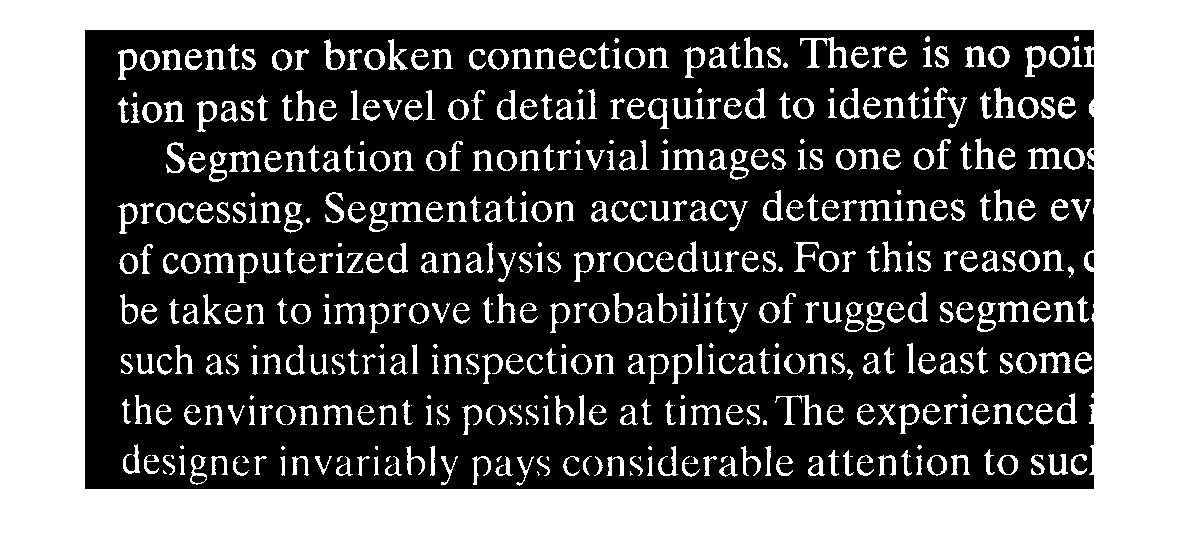
\includegraphics[width=\linewidth]{myfigure/p8/fig0929(a).png}
		\caption{}
		\label{fig:0929a}
	\end{subfigure}
	\begin{subfigure}[b]{0.45\linewidth}
    	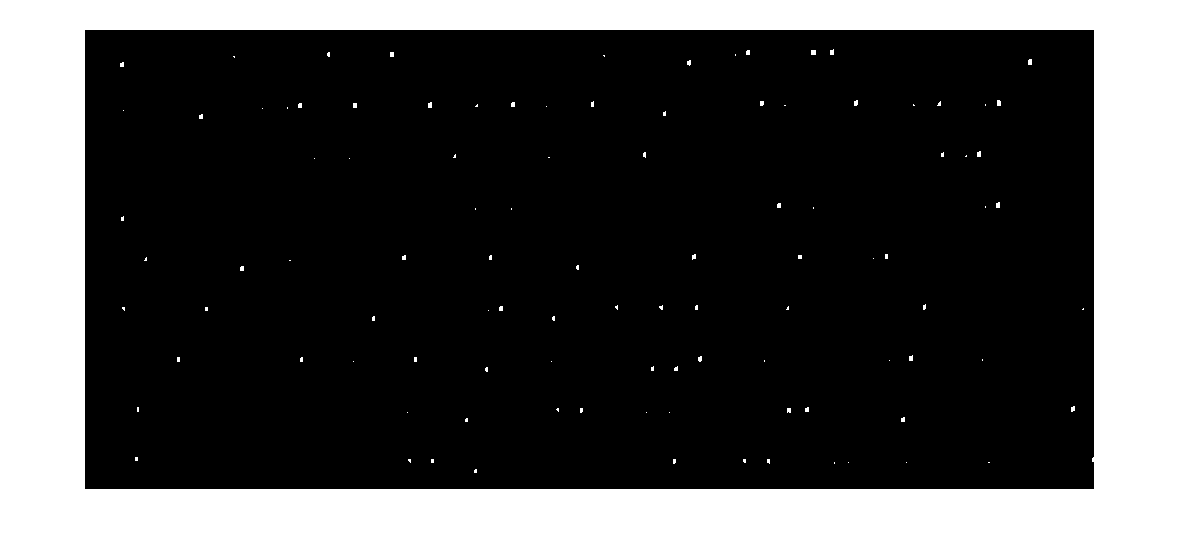
\includegraphics[width=\linewidth]{myfigure/p8/fig0929(b).png}
    	\caption{}
    	\label{fig:0929b}
  	\end{subfigure}
  	\begin{subfigure}[b]{0.45\linewidth}
		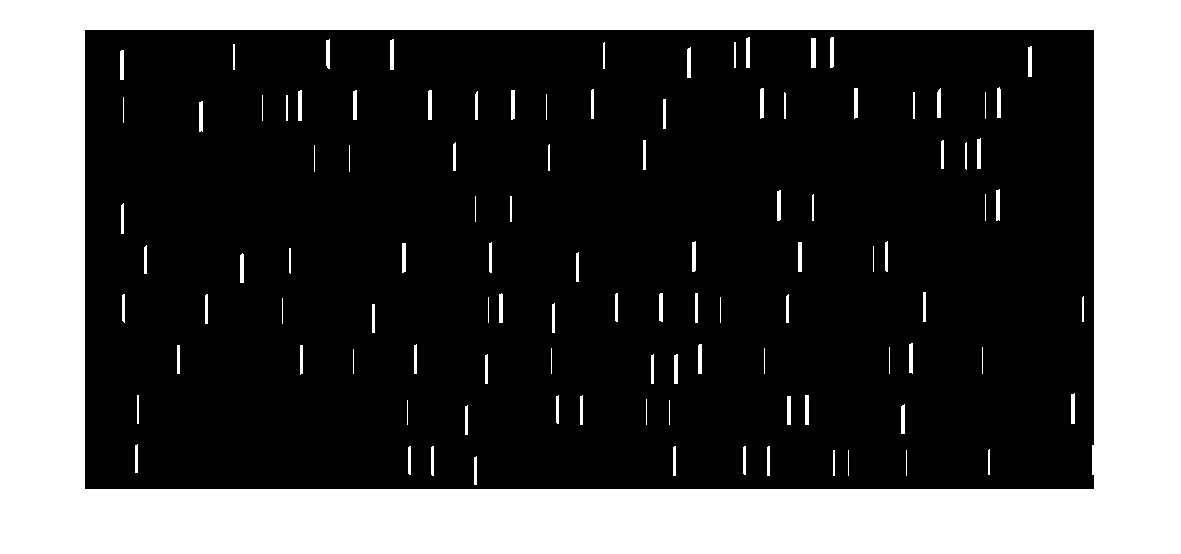
\includegraphics[width=\linewidth]{myfigure/p8/fig0929(c).png}
		\caption{}
		\label{fig:0929c}
	\end{subfigure}
	\begin{subfigure}[b]{0.45\linewidth}
    	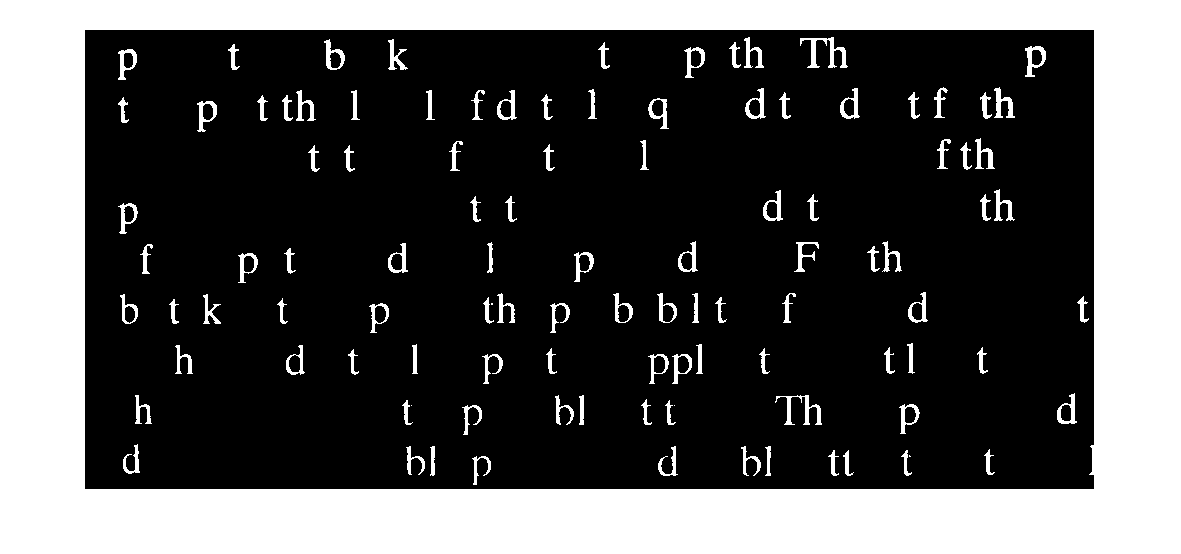
\includegraphics[width=\linewidth]{myfigure/p8/fig0929(d).png}
    	\caption{}
    	\label{fig:0929d}
  	\end{subfigure}
  	\caption{Task1-opening by reconstruction. (a)Original binary image $918 \times 2018$. (b)Erosion of (a) with a structuring element of size $51 \times 1$ pixels. (c)Opening of(a) with the structuring element $51 \times 1$, shown for comparison. (d)Result of opening by reconstruction.}
  	\label{fig:0929}
\end{figure}

The size of geodesic dilation reconstruction is $76$. This process cost about $7$ minutes. I output some of the intermediate results in Figure \ref{fig:0929append} that help us understand the reconstruction better.
\begin{figure}
	\centering
	\begin{subfigure}[b]{0.45\linewidth}
		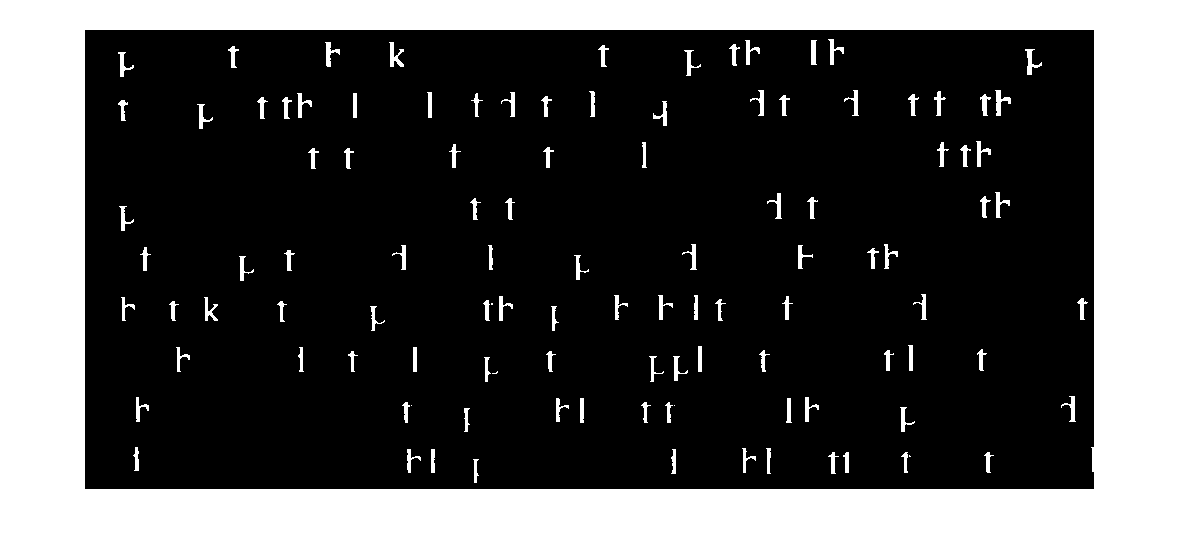
\includegraphics[width=\linewidth]{myfigure/p8/fig0929(d20).png}
		\caption{}
		\label{fig:0929d20}
	\end{subfigure}
	\begin{subfigure}[b]{0.45\linewidth}
    	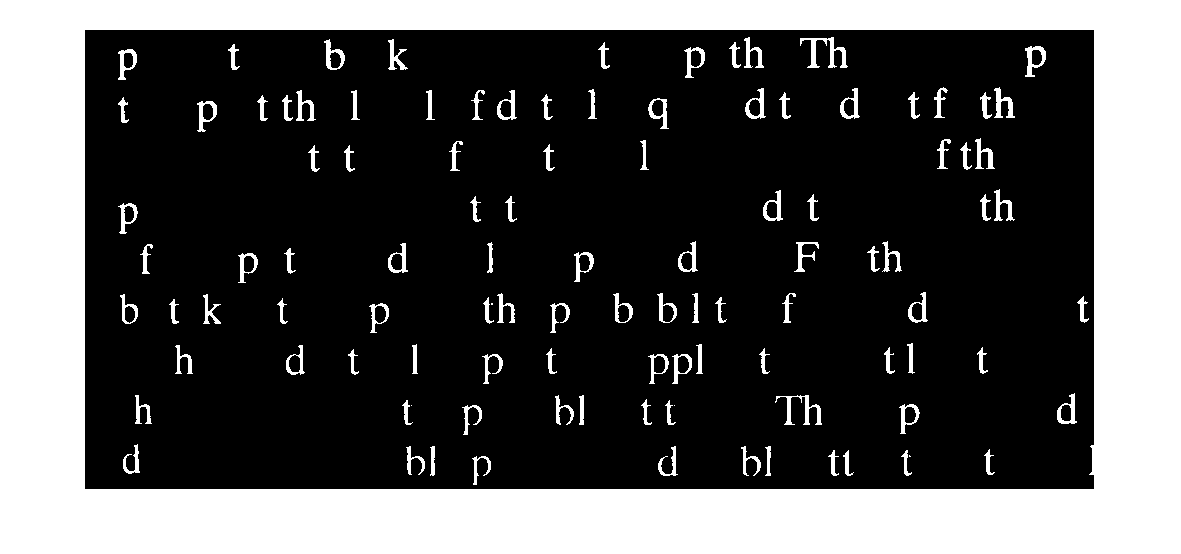
\includegraphics[width=\linewidth]{myfigure/p8/fig0929(d).png}
    	\caption{}
    	\label{fig:0929d76}
  	\end{subfigure}
	\caption{See task-1's process in details. (a)Dilation of size $20$. (b)Dilation of size $76$, the final results.}
  	\label{fig:0929append}
\end{figure}


\subsection{Task-2 Hole filling}
Here we develop a fully automated procedure based on morphological reconstruction. Let $I(x,y)$ denote a binary image and we form a marker $F$ that is $0$ everywhere, except at the image border; that is,
\begin{equation}
F(x, y)=\left\{
\begin{array}{rcl}
1-I(x,y) & \text{if $(x,y)$ is on the border of $I$} \\
0 & \text{otherwise} 
\end{array} \right.
\end{equation}
Then \begin{equation} H=\left[ R_{I^c}^D(F) \right]^c \end{equation} is a binary image equal to $I$ with all holes filled. \\
I use $3\time 3$ structuring element. The hole filling images are shown in Figure \ref{fig:0931}. A detailed process of dilation reconstruction with intermediate results are shown in Figure \ref{fig:0931append}. The reconstruction takes $479$ steps of dilation, which costs a very long period of about $40$ minutes. 
\begin{figure}[h!]
	\centering
	\begin{subfigure}[b]{0.45\linewidth}
		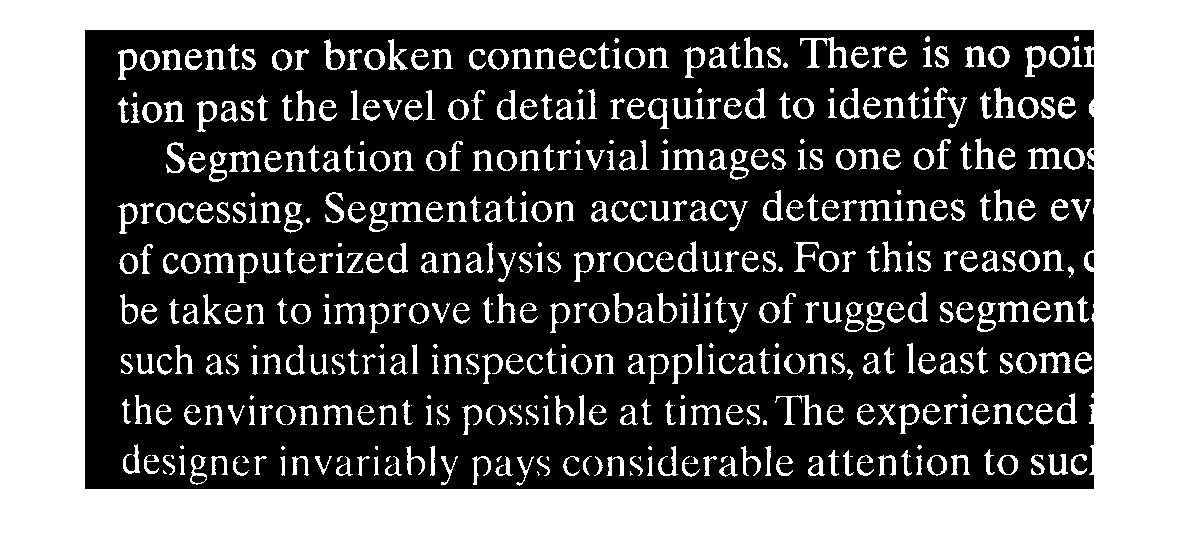
\includegraphics[width=\linewidth]{myfigure/p8/fig0929(a).png}
		\caption{}
		\label{fig:0931a}
	\end{subfigure}
	\begin{subfigure}[b]{0.45\linewidth}
    	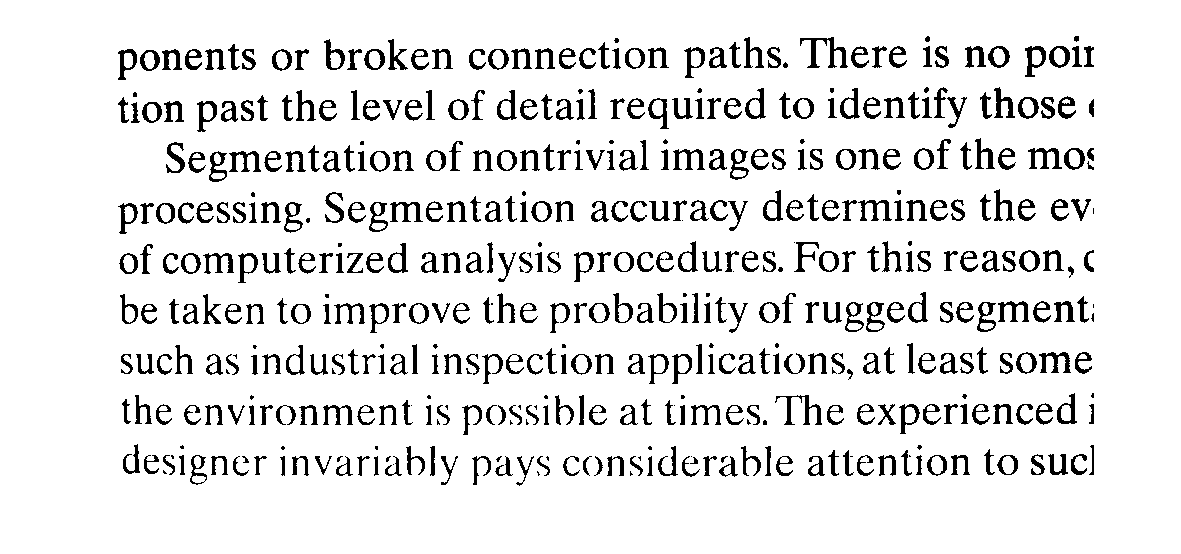
\includegraphics[width=\linewidth]{myfigure/p8/fig0931(b).png}
    	\caption{}
    	\label{fig:0931b}
  	\end{subfigure}
  	\begin{subfigure}[b]{0.45\linewidth}
		
\includegraphics[width=\linewidth]{myfigure/p8/fig0931(c).png}
		\caption{}
		\label{fig:0931c}
	\end{subfigure}
	\begin{subfigure}[b]{0.45\linewidth}
    	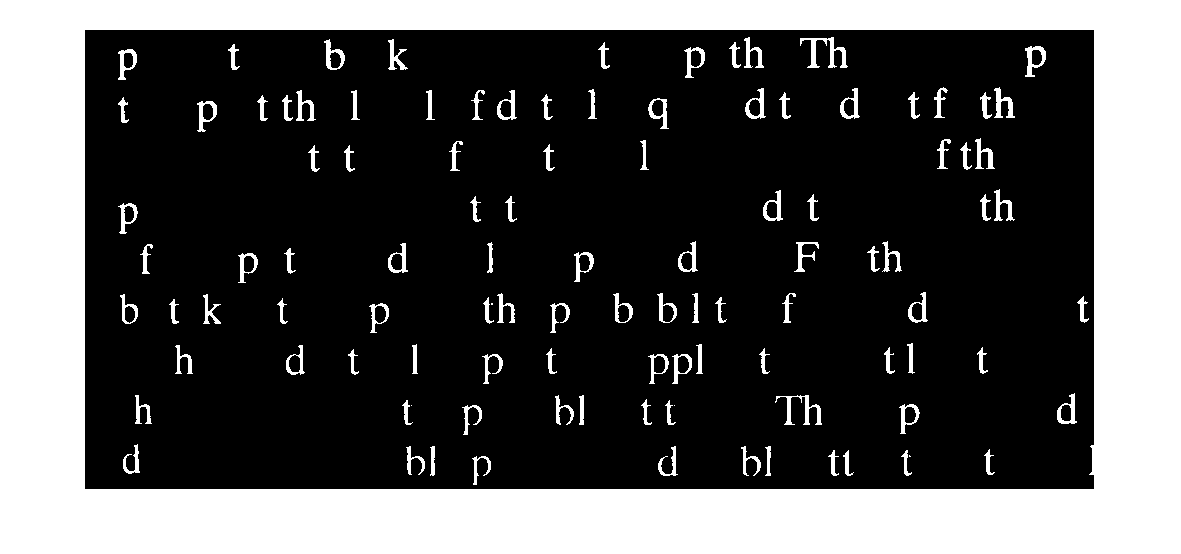
\includegraphics[width=\linewidth]{myfigure/p8/fig0929(d).png}
    	\caption{}
    	\label{fig:0931d}
  	\end{subfigure}
  	\caption{Task2-hole filling. (a)Original binary image $918 \times 2018$. (b)Complement of (a). Used as a mask. (c)Marker image. Seems like a whole black one, but in fact with some white on border. (d)Result of opening by reconstruction.}
  	\label{fig:0931}
\end{figure}

\begin{figure}[h!]
	\centering
	\begin{subfigure}[b]{0.45\linewidth}
		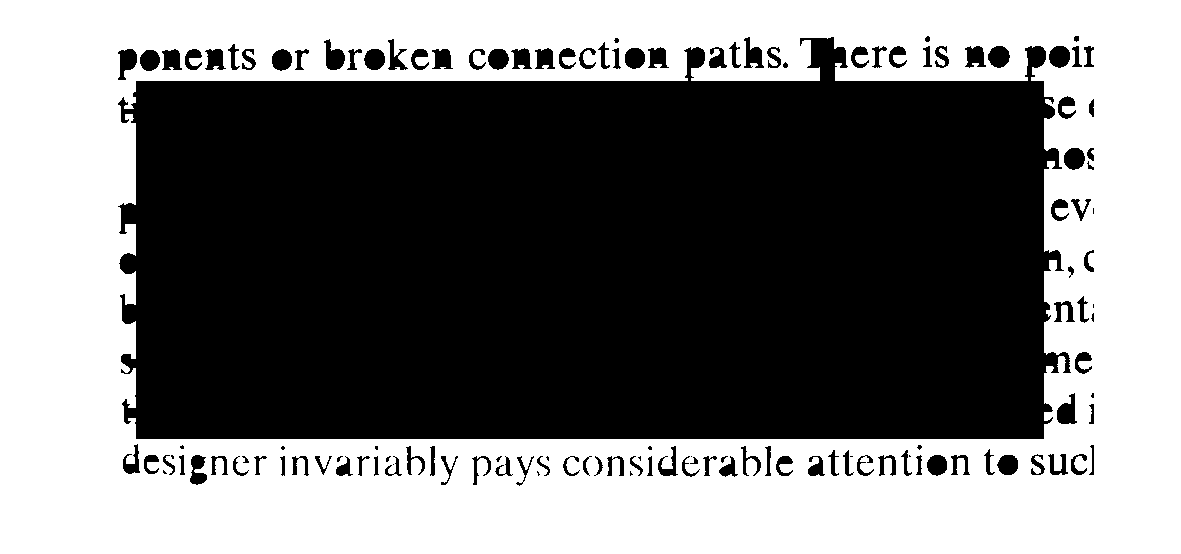
\includegraphics[width=\linewidth]{myfigure/p8/fig0931(d100).png}
		\caption{}
		\label{fig:0931d100}
	\end{subfigure}
	\begin{subfigure}[b]{0.45\linewidth}
    	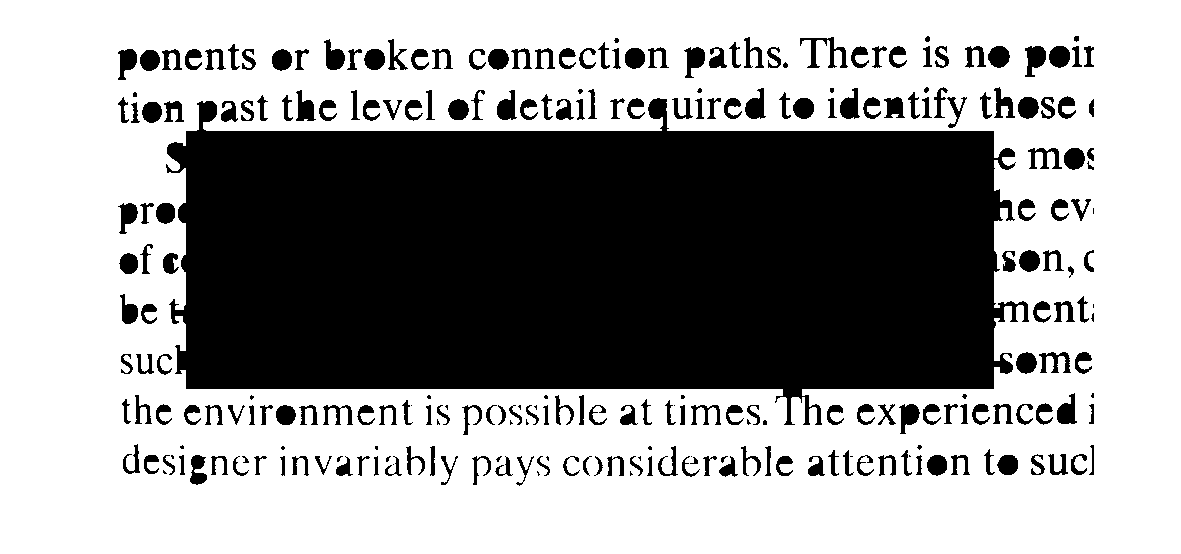
\includegraphics[width=\linewidth]{myfigure/p8/fig0931(d200).png}
    	\caption{}
    	\label{fig:0931d200}
  	\end{subfigure}
  	\begin{subfigure}[b]{0.45\linewidth}
		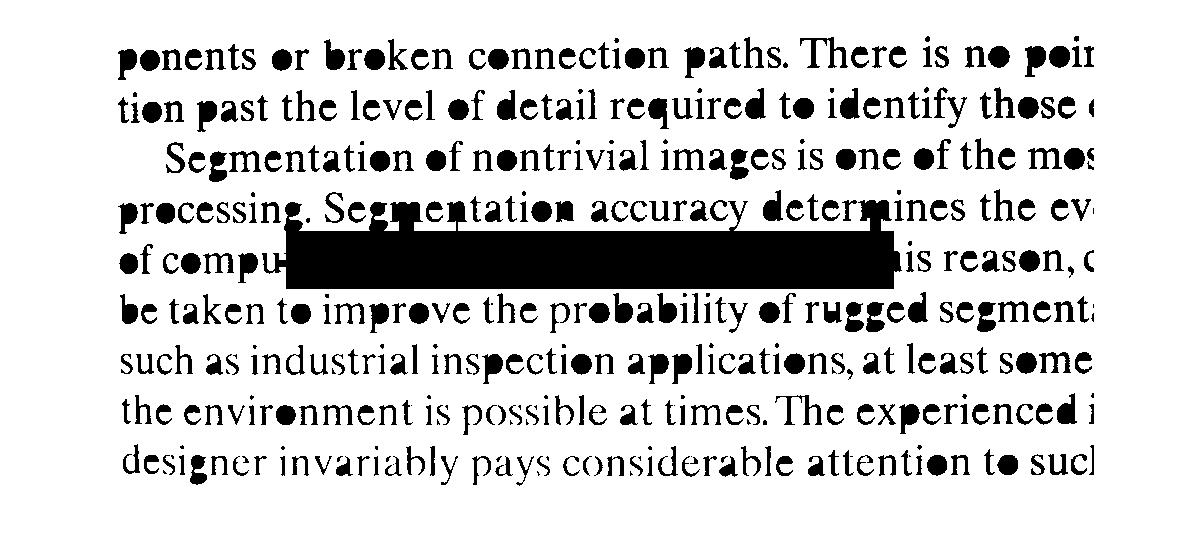
\includegraphics[width=\linewidth]{myfigure/p8/fig0931(d400).png}
		\caption{}
		\label{fig:0931d400}
	\end{subfigure}
	\begin{subfigure}[b]{0.45\linewidth}
    	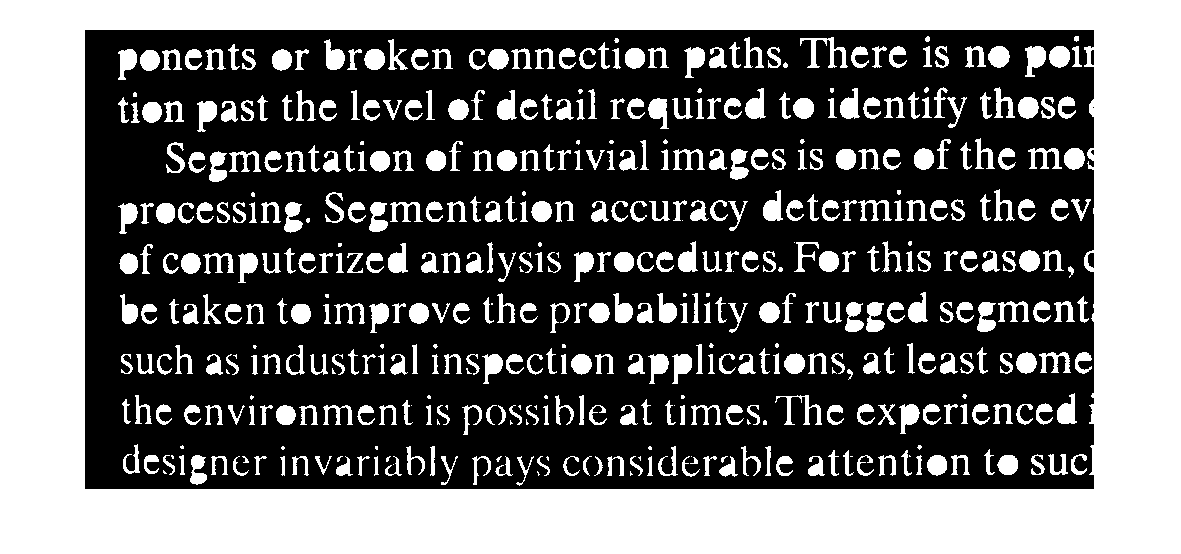
\includegraphics[width=\linewidth]{myfigure/p8/fig0931(d).png}
    	\caption{}
    	\label{fig:0931d479}
  	\end{subfigure}
  	\caption{The process of hole filling in details. (a)After 100 steps of dilation. (b)After 200 steps of dilation. (c)After 400 steps of dilation. Much closer to success! (d)The final result with completion.}
  	\label{fig:0931append}
\end{figure}


\subsection{Task-3 Border clearing}
Removing objects that touch the border is a useful work because it can screen images so that only complete objects remain for further processing. The marker $F(x,y)$ is defined as:
\begin{equation}  
F(x, y)=\left\{
\begin{array}{rcl}
I(x,y) & \text{if $(x,y)$ is on the border of $I$} \\
0 & \text{otherwise} \\
\end{array} \right.
\end{equation}
First we computes morphological reconstruction $R_I^D(F)$ and then computes the desired image $X$
\begin{equation} X=I-R_I^D(F) \end{equation}
I use structuring element of size $3 \times 3$. This task is much easier than task 2 and takes just $21$ steps of dilation in about $2$ minutes. Results are shown in Figure \ref{fig:0932}.
\begin{figure}[h!]
	\centering
  	\begin{subfigure}[b]{0.45\linewidth}
		
\includegraphics[width=\linewidth]{myfigure/p8/fig0932(a).png}
		\caption{}
		\label{fig:0932a}
	\end{subfigure}
	\begin{subfigure}[b]{0.45\linewidth}
    	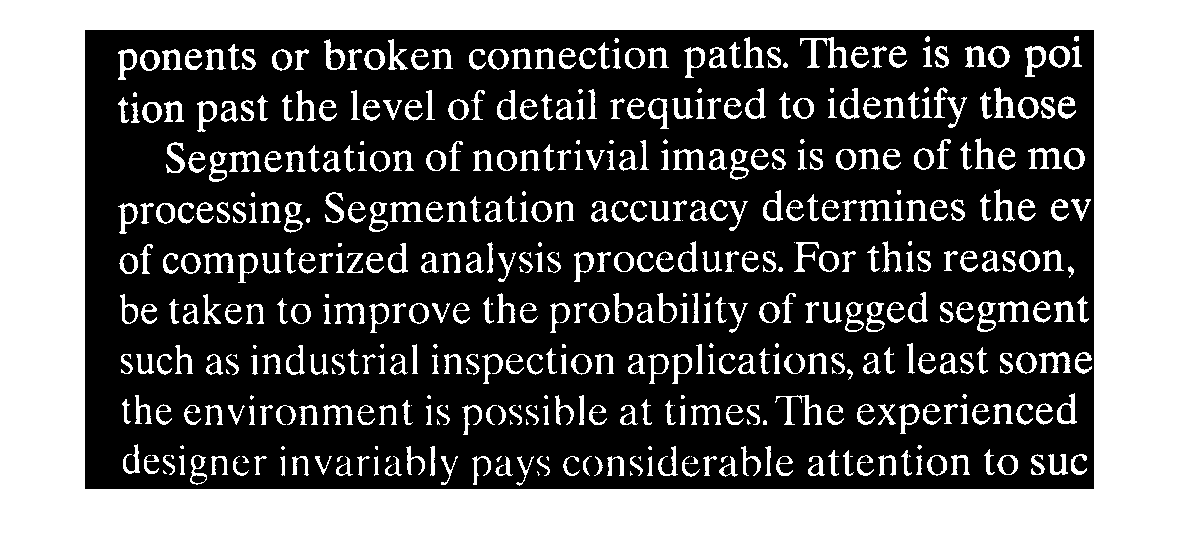
\includegraphics[width=\linewidth]{myfigure/p8/fig0932(b).png}
    	\caption{}
    	\label{fig:0932b}
  	\end{subfigure}
  	\caption{Border clearing. (a)After use border marker for 21-dilation reconstruction. The border letter. (b)The final result after subtraction.}
  	\label{fig:0932}
\end{figure}

\subsection{Implementation}
Matlab functions \emph{erosion, dilation, geodesic\_dilation, dilation\_reconstruction and opening\_reconstruction} are implemented for this project. I made a \textbf{mistake} on opening\_reconstruction at first that I still use $51 \times 1$ as the maker while calling dilation\_reconstruction. The wrong output image is the same as (c) as all the shorter horizontal adjacent relationship in our wanted characters was damaged. So for correction, we must use $3 \times 3$ as structuring element for dilation\_reconstruction called in opening\_reconstruction. \\
In the below code frame, I list the key part of these functions. Other process of calling these functions in main script are trivial so omitted here.\\
\lstset{language=Matlab}
\begin{lstlisting}
% key part of function erosion
for i = (1:M-m+1)
    for j = (1:N-n+1)
        x = imgf(i:i+m-1, j:j+n-1);
        if sum(sum(x.*B)) == m*n
            g(i+downshift, j+rightshift) = 1;
        end
    end
end

% key part of dilation_reconstruction 
k_times = 0;
while( ~isequal(f0, f1) )
    k_times = k_times + 1;
    f0 = f1;
    f1 = geodesic_dilation(f1, G, B);
end

% key part of geodesic_dilation
imgg = dilation(imgf, B) & G;

% key part of opening_reconstruction
for i=(1:n_size)
    f_erosion = erosion(f_erosion, B);
end
[imgg, k_times] = dilation_reconstruction(f_erosion, imgf, ones(3,3)); % here can not use ones(51, 1)
\end{lstlisting}

\subsection{Discussion}
These three tasks show the basic idea of morphological reconstruction used in feature extraction. We start from a marker which can be  obtained easily. Then we use the mask as the constrain to conduct set operations. More advanced topics are morphological operations on gray intensity images and image segmentation. This is a very interesting subproject.
The main obstacle here is \textbf{time}! I tried to do much vectorization but still have a big problem that 20-step-dilation cost about 2 minutes on the $918\times 2018$ image but the complexity is only about $918 \times 2018 \times 20 \times 9 \approx 4 \times 10^8$. I think the computation of this complexity need no more than 2 sec on language like C++ or python. However, I tried the matlab toolbox \emph{IPT} and it's just as fast as the expectation (within 2 sec). This is a strange but interesting problem.
